
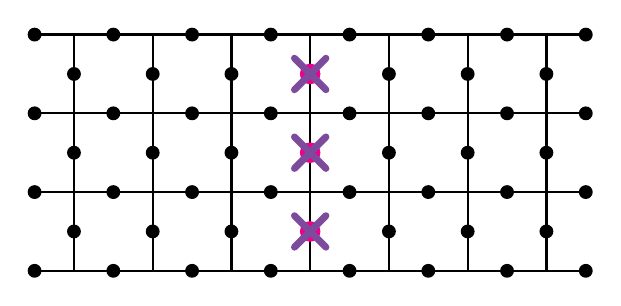
\begin{tikzpicture}[scale=1.0]
    % Define styles for nodes and edges
    \tikzset{
        blacknode/.style={circle, fill=black, inner sep=0pt, minimum size=5pt},
        pinknode/.style={circle, draw=magenta, fill=magenta, inner sep=0pt, minimum size=7pt},
        edge/.style={draw=black, thick}
    }
        \definecolor{crosscolor}{RGB}{125,75,155} % Purple

    % ==========================================
    % LEFT LATTICE
    % ==========================================
    % 1. Draw the underlying grid
    % Horizontal lines (x=0 to 3)
    \foreach \y in {0, 1, 2, 3} { \draw[edge] (-0.5,\y) -- (3,\y); } 
    % Vertical lines (x=0 to 2)
    \foreach \x in {0, 1, 2} { \draw[edge] (\x,0) -- (\x,3); } 

    % 2. Place black balls in the middle of horizontal edges
    \foreach \y in {0, 1, 2, 3} {
        \foreach \x in {-0.5, 0.5, 1.5, 2.5} {
            \node[blacknode] at (\x, \y) {};
        }
    }
    % 3. Place black balls in the middle of vertical edges
    \foreach \x in {0, 1, 2} {
        \foreach \y in {0.5, 1.5, 2.5} {
            \node[blacknode] at (\x, \y) {};
        }
    }

    % ==========================================
    % RIGHT LATTICE
    % ==========================================
    % Shifted left so it meets the left lattice perfectly
    
    % 1. Draw the underlying grid
    % Horizontal lines (x=3 to 6) - Now touching the left lattice at x=3
    \foreach \y in {0, 1, 2, 3} { \draw[edge] (3,\y) -- (6.5,\y); } 
    % Vertical lines (x=4 to 6)
    \foreach \x in {3, 4, 5, 6} { \draw[edge] (\x,0) -- (\x,3); } 

    % 2. Place black balls in the middle of horizontal edges
    \foreach \y in {0, 1, 2, 3} {
        \foreach \x in {3.5, 4.5, 5.5, 6.5} {
            \node[blacknode] at (\x, \y) {};
        }
    }
    % 3. Place black balls in the middle of vertical edges
    \foreach \x in {4, 5, 6} {
        \foreach \y in {0.5, 1.5, 2.5} {
            \node[blacknode] at (\x, \y) {};
        }
    }

    % ==========================================
    % CENTRAL PINK COLUMN
    % ==========================================
    % Placed precisely at x=3, sitting right on top of the touching horizontal edges
    \foreach \y in {0.5, 1.5, 2.5} {
        \node[pinknode] at (3, \y) {};
    }

        \foreach \y in {0.5, 1.5, 2.5} {
        \draw[crosscolor, line width=2.5pt, line cap=round] (3-0.2, \y-0.2) -- (3+0.2, \y+0.2);
        \draw[crosscolor, line width=2.5pt, line cap=round] (3-0.2, \y+0.2) -- (3+0.2, \y-0.2);
    }

\end{tikzpicture}